\documentclass[11pt, spanish, a4paper, twoside]{article}

% Versión 1.er cuat 2021 Víctor Bettachini < vbettachini@unlam.edu.ar >

\usepackage[T1]{fontenc}
\usepackage[utf8]{inputenc}

\usepackage[spanish, es-tabla]{babel}
% \def\spanishoptions{argentina} % Was macht dass?
% \usepackage{babelbib}
% \selectbiblanguage{spanish}
% \addto\shorthandsspanish{\spanishdeactivate{~<>}}


\usepackage{graphicx}
\graphicspath{{./figuras/}{../LaTeX/}{../figurasLaTeX/}{./figs}}
% \usepackage{float}

\usepackage[arrowdel]{physics}
\newcommand{\pvec}[1]{\vec{#1}\mkern2mu\vphantom{#1}}
% \usepackage{units}
\usepackage[separate-uncertainty= true, multi-part-units= single, range-units= single, range-phrase= {~a~}, locale= FR]{siunitx}
\usepackage{isotope} % $\isotope[A][Z]{X}\to\isotope[A-4][Z-2]{Y}+\isotope[4][2]{\alpha}

\usepackage{tasks}
\usepackage[inline]{enumitem}
% \usepackage{enumerate}

\usepackage{hyperref}

% \usepackage{amsmath}
% \usepackage{amstext}
% \usepackage{amssymb}

\usepackage{tikz}
\usepackage{tikz-3dplot}
\usepackage{tikz-dimline}
\usetikzlibrary{calc}
% \usetikzlibrary{math}
\usetikzlibrary{arrows.meta}
\usetikzlibrary{snakes}
\usetikzlibrary{decorations}
\usetikzlibrary{decorations.pathmorphing}
\usetikzlibrary{patterns}

\usepackage[hmargin=1cm,vmargin=3cm, top= 0.75cm,nohead]{geometry}

\usepackage{lastpage}
\usepackage{fancyhdr}
\pagestyle{fancyplain}
\fancyhf{}
\setlength\headheight{28.7pt} 
\fancyhead[LE, LO]{\textbf{Mecánica Analítica Computacional} }
% \fancyhead[LE, LO]{\textbf{Mecánica General} }
\fancyhead[RE, RO]{\href{https://ingenieria.unlam.edu.ar/}{$\vcenter{\hbox{
\includegraphics[height=1cm]{ambos.pdf}}}$}}
\fancyfoot{\href{https://creativecommons.org/licenses/by-nc-sa/4.0/deed.es_ES}{$\vcenter{\hbox{
\includegraphics[height=0.4cm]{by-nc-sa_80x15.pdf}}}$} \href{https://ingenieria.unlam.edu.ar/}{DIIT - UNLaM}}
\fancyfoot[C]{ {\tiny Actualizado al \today} }
\fancyfoot[RO, LE]{Pág. \thepage/\pageref{LastPage}}
\renewcommand{\headrulewidth}{0pt}
\renewcommand{\footrulewidth}{0pt}

% LTeX: language = es-AR

\begin{document}
\begin{center}
  % \textsc{\large Mecánica general}\\
  \textsc{\large Cuerpo rígido | Tensores de inercia}
\end{center}

% De poder resolver estos problemas en forma autónoma puede asumir que adquirió los conocimientos mínimos sobre los temas abordados en la semana. No dude en consultar a docentes y compañeros si no puede terminarlos.
% Los problemas marcados con (*) son opcionales.

\begin{enumerate}

	\item 
	\begin{minipage}[t][6cm]{0.65\textwidth}
		\textbf{Péndulo de torsión desbalanceado}\\
		El sistema que se muestra en la ilustración para \(t=0\) presenta pesos en los extremos de dos brazos.
		La barra dispuesta verticalmente se mantiene en tal dirección con rulemanes que posibilitan que el eje rote sin fricción con velocidad angular $\Omega$ constante respecto el marco inercial $O_{xyz}$.
		Para este análisis la masa de brazos y ejes es despreciable frente a la de los pesos \(m\).
		Calcule: 
		\begin{tasks} 
			\task tensor de inercia respecto a A en función del tiempo \(\overline{\overline{I}}_A(t)\)\\
			\task momento angular $\vec{L}_A (t) = \overline{\overline{I}}_A (t) \vec{\Omega}$ y torque $\vec{\tau} (t) = \dot{\vec{L}} (t)$.
		\end{tasks}
	\end{minipage}
	\begin{minipage}[c][0cm][t]{0.3\textwidth}
		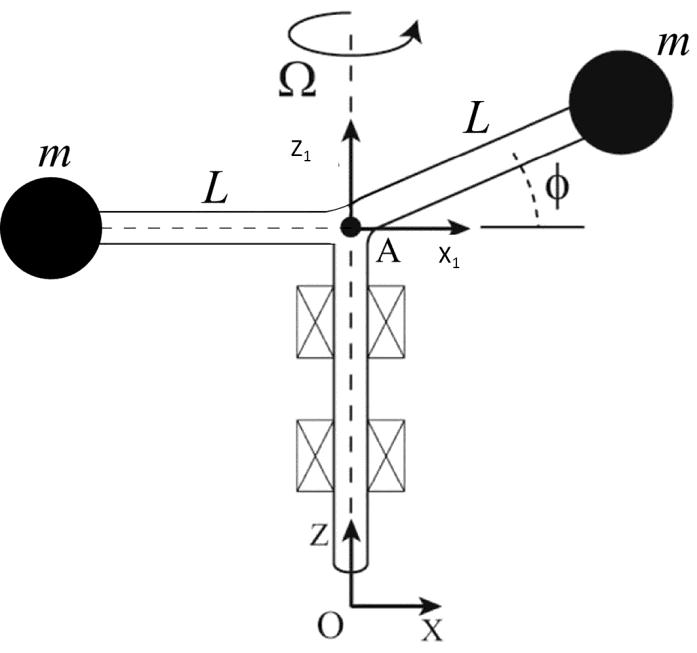
\includegraphics[width=\textwidth]{o-021}
	\end{minipage}
	Resultados:\\
			\[
				\scalebox{0.8}{$
				\overline{\overline{I}}_A = \left[\begin{matrix}\ell^{2} m \left(- \cos^{2}{\left(\phi \right)} \cos^{2}{\left(\Omega t \right)} - \cos^{2}{\left(\Omega t \right)} + 2\right) & - \ell^{2} m \left(\cos^{2}{\left(\phi \right)} + 1\right) \sin{\left(\Omega t \right)} \cos{\left(\Omega t \right)} & \frac{\ell^{2} m \left(\sin{\left(\Omega t - 2 \phi \right)} - \sin{\left(\Omega t + 2 \phi \right)}\right)}{4}\\- \ell^{2} m \left(\cos^{2}{\left(\phi \right)} + 1\right) \sin{\left(\Omega t \right)} \cos{\left(\Omega t \right)} & \ell^{2} m \left(\sin^{2}{\left(\phi \right)} \sin^{2}{\left(\Omega t \right)} - 2 \sin^{2}{\left(\Omega t \right)} + 2\right) & - \frac{\ell^{2} m \left(\cos{\left(\Omega t - 2 \phi \right)} - \cos{\left(\Omega t + 2 \phi \right)}\right)}{4}\\\ell^{2} m \left(\cos^{2}{\left(\phi \right)} + 1\right) & - \frac{\ell^{2} m \left(\cos{\left(\Omega t - 2 \phi \right)} - \cos{\left(\Omega t + 2 \phi \right)}\right)}{4} & \ell^{2} m \left(\cos^{2}{\left(\phi \right)} + 1\right)\end{matrix}\right]
				$}
				\] 
			\[
				\vec{L}_A = \left[\begin{matrix}\frac{\Omega \ell^{2} m \left(\sin{\left(\Omega t - 2 \phi \right)} - \sin{\left(\Omega t + 2 \phi \right)}\right)}{4}\\- \frac{\Omega \ell^{2} m \left(\cos{\left(\Omega t - 2 \phi \right)} - \cos{\left(\Omega t + 2 \phi \right)}\right)}{4}\\\Omega \ell^{2} m \left(\cos^{2}{\left(\phi \right)} + 1\right)\end{matrix}\right]
			\qquad
				\vec{\tau}_A = \left[\begin{matrix}\frac{\Omega^{2} \ell^{2} m \left(\cos{\left(\Omega t - 2 \phi \right)} - \cos{\left(\Omega t + 2 \phi \right)}\right)}{4}\\\frac{\Omega^{2} \ell^{2} m \left(\sin{\left(\Omega t - 2 \phi \right)} - \sin{\left(\Omega t + 2 \phi \right)}\right)}{4}\\0\end{matrix}\right]
			\]

	\item 
	\begin{minipage}[t][3.5cm]{0.73\textwidth}
		\textbf{Molécula de agua}\\
		Calcule los momentos de inercia en el SI para una molécula de \isotope{H_2O}.
		En CNPT se abre con un ángulo de \ang{104,5;;} y median \SI{95.84}{\pico\metre} entre \isotope{O} y \isotope{H}.
		Resultado:\\
		\[
			\scalebox{0.8}{$
			\overline{\overline{I}} = \left[\begin{matrix}1.02353565118967 \cdot 10^{-47} & 0 & 0\\0 & 1.92240664746526 \cdot 10^{-47} & 0\\0 & 0 & 2.94594229865493 \cdot 10^{-47}\end{matrix}\right]
			$}	
		\]
	\end{minipage}
	\begin{minipage}[c][2cm][t]{0.2\textwidth}
		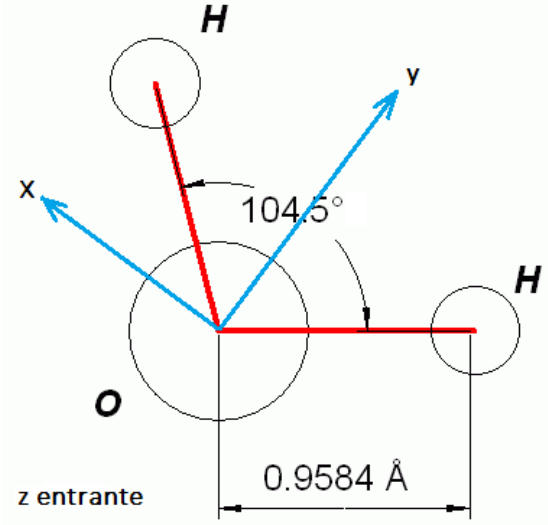
\includegraphics[width=\textwidth]{moleculaH2O}
	\end{minipage}


	\item
	\textbf{Componentes del tensor de inercia para una barra}\\
	Se tiene una barra de \(m= \SI{1}{\kilo\gram}\) de sección despreciable frente a \(l= \SI{1}{\metre}\).
	De alinear un eje (\(\hat{z}\)) con ella, 
	\begin{tasks}(2)
		\task	Calcule sus momentos de inercia.
		\task Muestre que sucede con los productos de inercia. 
	\end{tasks}


	\item
	\textbf{Ejes conveniente para el cálculo del momentos de inercia}\\
	Se dibujan vistas en perspectiva de diversos objetos.
	Sobre estos dibuje los ejes intersectando en el punto más conveniente para el cálculo de momentos de inercia, esto es, en el centro de masa.
	Haga lo mismo con los dos ejes que corresponden a la proyección en planta.
	\vspace{-0.8cm}
	\begin{tasks}(4)
		\task 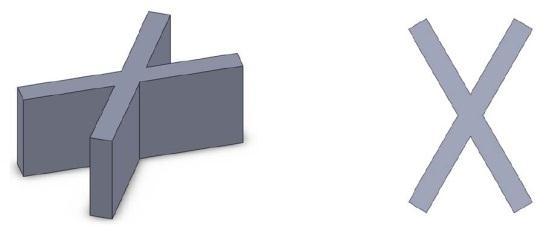
\includegraphics[width=0.15\textwidth]{o-000}
		\task 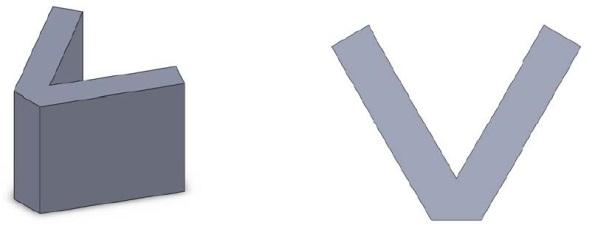
\includegraphics[width=0.15\textwidth]{o-001}
		\task 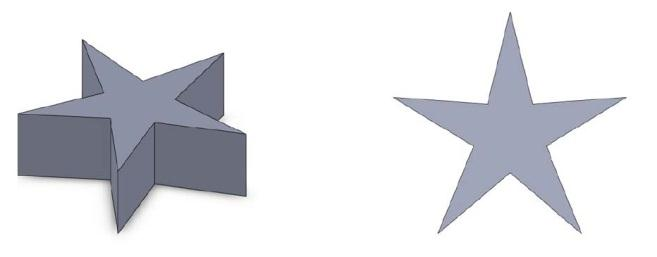
\includegraphics[width=0.15\textwidth]{o-002}
		\task 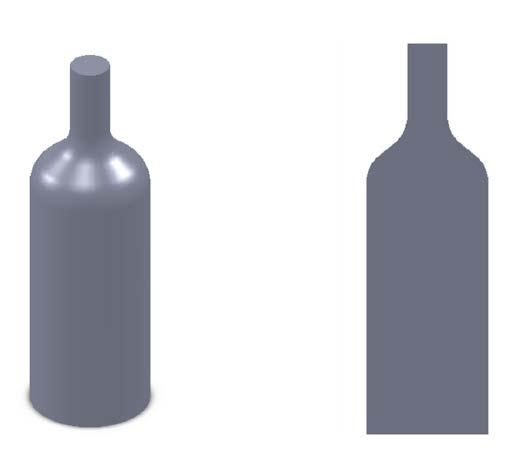
\includegraphics[width=0.15\textwidth]{o-003}
	\end{tasks}


	\end{enumerate}

\end{document}
